\section{Simulations and Performance Analysis}
In this section we describe the implementation of our simulator and discuss some performance measurements acquired using this tool. We also describe features that should be added to the simulator to support more realistic experiments. We conclude with a discussion of good parameter selection based on our observations using the simulator.

\subsection{Simulation Design}
To assess the expected overhead introduced by Boomerang we implemented a custom discrete-time simulator that emulates the behavior of Bitcoin nodes (software clients) running Boomerang. Time in the simulation is measured in epochs; at every epoch a series of events occurs that advances the state of the system in some (usually) deterministic way. Our simulator supports the following behavior to closely resemble Boomerang:
\begin{enumerate}
	\item Nodes enter and exit the network at random times. 
	\item Nodes make new transactions using configuration-specificed parameters $W$ and $D$ at a random rate $\pi$.
	\item Nodes generate cover traffic at a random rate $\sigma$.
	\item Nodes manage their internal address address books according the protocol described in section \ref{sec:design}.
\end{enumerate}

In addition, the simulation dynamically computes the following performance metrics:
\begin{enumerate}
	\item Average number of ``computations'' done per node (i.e., the number of public-key encryption operations to encode a transaction).
	\item Total and average message latency from the start to end of a circuit for single and every message, respectively.
	\item Node forwarding throughput (messages/s).
	\item Number of completed messages (transactions and cover messages) vs the number of in-progress messages.
	\item Average number of transaction broadcast retries per node.
\end{enumerate}

The parameters for a particular simulation are specified via a YAML configuration file which is parsed using the Java-based JYaml library \cite{jyaml}. An example configuration file which creates a simulation with $N = 100$ nodes, $D = 6$, $W = 2$, and cover and transaction generation rates uniformly distributed between $[1, 5000]$ and $[1, 7500]$ epochs (i.e., the most granular unit of time).

\begin{lstlisting}
simTime: 2500
numNodes: 100
enterRate: 750
exitRate: 750
gridHeight: 10000
gridWidth: 10000
chaffGenRate: 5000
txGenRate: 7500
circuitWidth: 2
circuitDepth: 6
retryLimit: 7500
buffSize: 10
mixDelay: 50
pktSize: 1024
initialAddressSize: 250
validNodeTransmitReq: 50
addressBookSize: 1000
seed: 256
outfileprefix: "config-out"
path: "."
genMatrices: false
keepInMemory: false
\end{lstlisting}

The {\tt genMatrices} and {\tt keepInMemory} flags are used to ensure that the Java heap space isn't exhausted from memory leaks by storing all of the events generated by the simulation at each time epoch. To run the simulation with 8GB of heap space on the example configuration listed above, which is stored in a local file {\tt config.yaml}, one would run the following command:

\begin{center}
{\small \tt java -cp ./jyaml-1.3.jar:. -Xmx8g Boomerang config.yaml}
\end{center}

\subsection{Performance Metrics}
Using our simulation, we performed a series of small and large experiments with properties summarized in Table \ref{tab:experiments}. Due to physical memory limitations and the initial single-threaded nature design of our simulator, we could not conduct experiments beyond $N \approx 25000$. We will address this shortcoming in our simulation design for future work.

TODO: discuss the graphs/charts here

\begin{table*}
\begin{center}
\caption{TODO}
\label{tab:sim-results}
    \begin{tabular}{|c|c|c|c|c|c|} \hline
    {\bf Experiment \#} & $N$ & $D$ & $W$ & $\sigma_{max}$ & $\pi_{max}$ \\ \hline
    1 & 50     & 6 & 2 & 5000 & 7500 \\ 
    2 & 100    & 6 & 2 & 5000 & 7500 \\ 
    3 & 150    & 6 & 2 & 5000 & 7500 \\ 
    4 & 200    & 6 & 2 & 5000 & 7500 \\ 
    5 & 250    & 6 & 2 & 5000 & 7500 \\ 
    6 & 1000   & 6 & 2 & 5000 & 7500 \\ 
    7 & 10000  & 6 & 2 & 5000 & 7500 \\ 
    8 & 50     & 8 & 1 & 5000 & 15000 \\ 
    9 & 100    & 8 & 1 & 5000 & 15000 \\ 
    10 & 150   & 8 & 1 & 5000 & 15000 \\ 
    11 & 200   & 8 & 1 & 5000 & 15000 \\ 
    12 & 250   & 8 & 1 & 5000 & 15000 \\ 
    13 & 1000  & 8 & 1 & 5000 & 15000 \\ 
    14 & 10000 & 8 & 1 & 5000 & 15000 \\ 


    \hline
    \end{tabular}
\end{center}
\end{table*}

\begin{table*}
\begin{center}
\caption{TODO}
\label{tab:sim-results}
    \begin{tabular}{|c|c|c|c|c|c|} \hline
    {\bf Experiment \#} & {\bf E[Message Latency]} & {\bf E[Chaff Encryptions]} & {\bf E[Transaction Encryptions]} & {\bf E[Forwarded Messages]} & {\bf E[Retries]} \\ \hline
    1 & ~ & ~ & ~ & ~ & ~ \\ 
    2 & ~ & ~ & ~ & ~ & ~ \\ 
    3 & ~ & ~ & ~ & ~ & ~ \\ 
    4 & ~ & ~ & ~ & ~ & ~ \\ 
    5 & ~ & ~ & ~ & ~ & ~ \\ 
    6 & ~ & 35.25 & 18.91 & 16468.7 & 0.04 \\
    7 & ~ & 29.59 & 20.75 & 13750.8 & 0.02 \\ \hline
    \end{tabular}
\end{center}
\end{table*}

\begin{figure*}[ht!]
\begin{center}
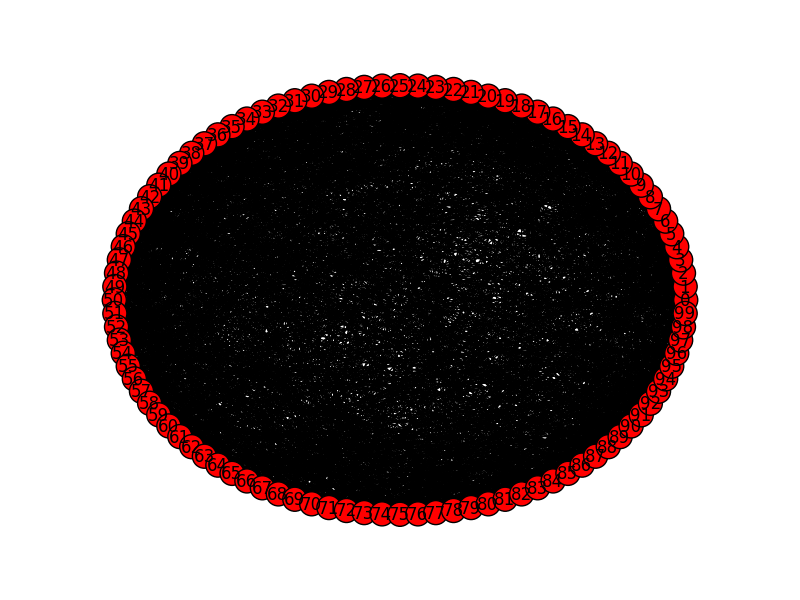
\includegraphics[scale=0.5]{./images/sim1_completedMessage_complete.png}
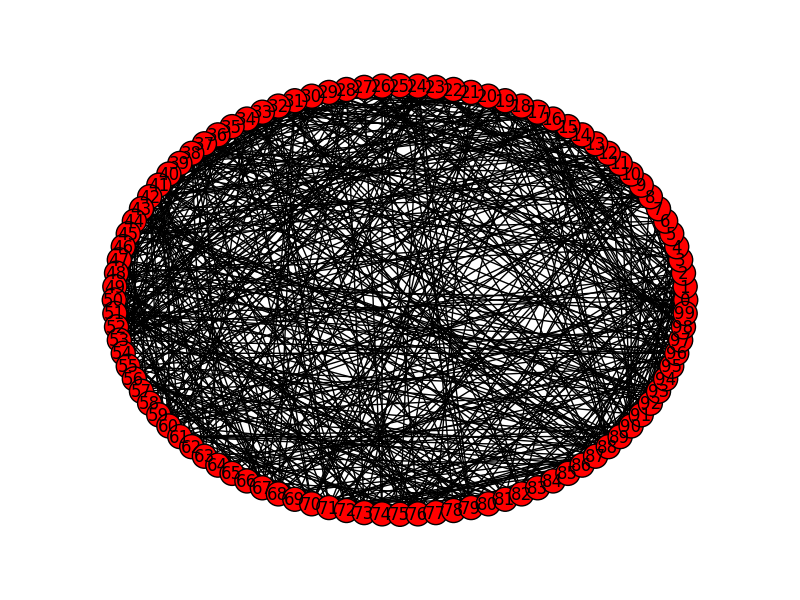
\includegraphics[scale=0.5]{./images/sim1_completedMessage_tx.png}
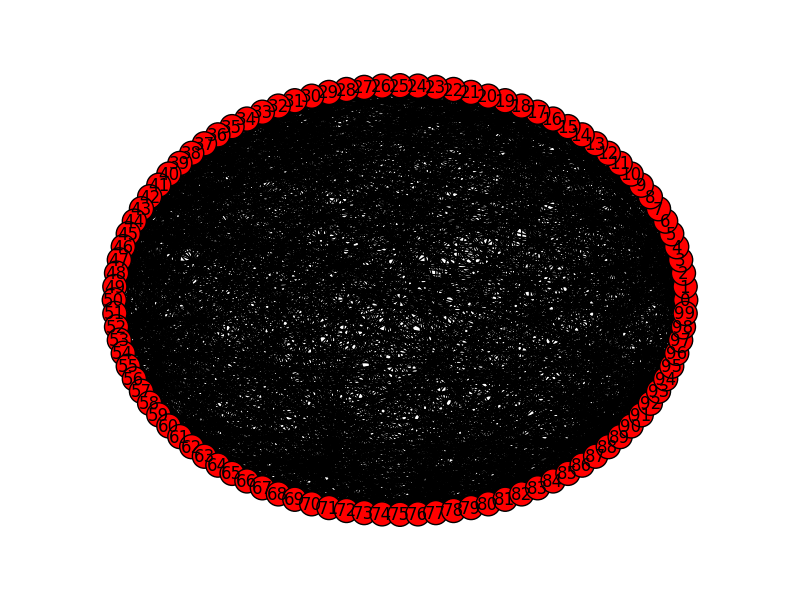
\includegraphics[scale=0.5]{./images/sim1_completedMessage_chaff.png}
\caption{The top figure shows the flow of both dummy messages and forwarded transactions from Experiment \#1, the middle figure shows only the transaction messages, and the bottom figure shows the cover traffic. Nodes have directed edges between them if some message was sent between them during the lifetime of the simulation. The coverage of nodes is clearly uniformly distributed, as desired.}
\label{fig:boomerang_message}
\end{center}
\end{figure*}

\subsection{Parameter Selection}

From a performance perspective, our main goal is to minimize the overhead of Boomerang message encoding, transmission, and forwarding while maximizing the anonymity properties discussed in the previous section. To that end, we discuss how the performance varies based on system-wide parameters that influence such anonymity properties. Based on the Boomerang design it is clear that the performance of the Boomerang scheme is tightly coupled to $W$, $D$, and the rate at which cover traffic and new encoded transactions generation.

Using the custom simulator developed for this project, we propose ****

% cover traffic generation rate (random variable)
% mix buffer delay (random variable)
% circuit length (fixed)
% mix buffer size (fixed)
% encoded transaction size

